\documentclass[10pt,letterpaper]{article}
\usepackage[margin=0.85in]{geometry}
\usepackage[T1]{fontenc}
\usepackage{iftex}
\ifPDFTeX
  \usepackage[utf8]{inputenc}
\fi
\usepackage{amsmath,amssymb}
\usepackage{booktabs,array,graphicx}
\usepackage{xcolor}
\usepackage[round,authoryear]{natbib}
\usepackage{xurl}
\usepackage{hyperref}

\definecolor{placeholdercolor}{RGB}{135,45,20}
\hypersetup{
  colorlinks=true,
  linkcolor=blue,
  citecolor=blue,
  urlcolor=blue,
  pdftitle={Remove or Reset Before LoRA? Memory, SQL Performance, and Broader Behavior in a Gemma 3 4B Case Study},
  pdfauthor={Adit Hasan}
}
\newcommand{\todo}[1]{%
  \par\smallskip\noindent
  {\color{placeholdercolor}\textbf{[PLACEHOLDER]} #1}%
  \par\smallskip}
\newcommand{\tbd}{\textit{TBD}}
\newcommand{\repositoryurl}{https://github.com/adhasan-dev/remove-or-reset}
\newcommand{\E}{\mathbb{E}}
\DeclareRobustCommand{\dataset}[1]{\hyperlink{dataset-#1}{\textnormal{#1}}}
\newcommand{\datasetentry}[1]{\hypertarget{dataset-#1}{\textnormal{#1}}}
\setlength{\parskip}{2pt}
\setlength{\emergencystretch}{2em}
\setlength{\bibsep}{3pt}
\renewcommand{\arraystretch}{1.08}

\title{Remove or Reset? A Case Study of Channel Selection\\
Before LoRA Fine-Tuning}
\author{Adit Hasan\\
\small Independent Researcher}
\date{Preprint --- 20 November 2026}

\begin{document}
\maketitle

\begin{abstract}
General purpose Large Language Models (LLMs) are powerful but computationally expensive.
In the context LoRA specialization, the model might have encoded knowledge
and capabilities that are not relevant to the target task. This raises the question of whether
we can remove or reset selected channels in the model's MLP layers before fine-tuning and still
achieve comparable specialized task performance and efficiency.
This study explores LoRA fine-tuning performance along two dimensions: First, how does removing selected
MLP channnels from the model compare to resetting them? Second, how do different strategies
for selecting channels to remove/reset perform in this context? We studied the pretrained 
Gemma 3 4B text model, with text-to-SQL as the specialization task, comparing ordinary LoRA 
with LoRA applied after removing or resetting 20\% of its MLP channels. Across three 
matched training seeds, quota-free guided removal reduced the native parameter count by 13.78\% and peak 
allocated training memory by 10.5-10.8\%. On the same 128 SQL queries, mean execution 
agreement was 72.4\% for the compact model and 74.5\% for ordinary LoRA.
A short-answer cross-domain screen (\dataset{D06}) yielded 53.9\% accuracy for ordinary LoRa and 
44.7\% for quota-free guided removal, implying guided removal did not retain as much of 
the original general capabilities after adaptation. Single-seed comparisons with matched 
channel resets found no consistent SQL benefit from retaining full width. In this setting, 
channel removal produced a smaller SQL specialist with repeatable training-memory savings 
and a modest average target-task gap.
\end{abstract}

\section{Introduction}
\label{sec:introduction}

The success of LLMs lies in their billions to trillions of parameters and
pretaining on trillions of tokens, giving rise to impressive general-purpose capabilities.
Specialization need not preserve every behavior of a general-purpose model, but those generalized
capabilities may or may not contribute to the performance of specialized tasks.
The practical question here is how removing or resetting selected channels in the MLP layers 
\emph{before} LoRA fine-tuning affects the target-task outcome and resource usage. 
Physical channel removal reduces dense tensor dimensions and can reduce
resource requirements; practical training and inference speedups are not
established by this study. Resetting keeps those dimensions but replaces
selected incoming weights and zeroes their outgoing contribution, potentially 
giving LoRA "more room" to adapt. These operations need not have the same
adaptation dynamics, even when they initially suppress the same channels.

We separate two questions. One question relates to the method used to
select which channels to remove/reset. For a fixed operation and channel budget,
does a selector that protects channels useful across calibration tasks aid
subsequent \emph{target-task adaptation}, compared with random or
retained-loss Taylor selection? Second, for the same selected channels,
does retaining reset pathways improve adaptation enough to justify the
full-width model? Broad calibration utility is a proposed predictor of useful
adaptation capacity, not an assumption that all specialists need broad
general ability.

\paragraph{Falsifiable expectations.}
The selection hypothesis predicts higher post-LoRA target-task execution
agreement for guided selection than for its uniform-allocation random and
Taylor controls. Equal or worse agreement, or paired uncertainty that leaves
the proposed benefit unresolved, would weaken evidence for that hypothesis.
The reset hypothesis predicts a target-task benefit over same-mask removal;
its practical assessment must also account for retained parameter and resource
costs. No equivalence or non-inferiority margin was established for this study.

The executed instance is one pretrained model, one specialization domain (SQL),
and a small fixed SQL evaluation panel (\dataset{D05}). The original nine-arm
comparison uses seed 42; ordinary LoRA and quota-free guided removal additionally
use matched seeds 43 and 44 (\autoref{sec:seed-replication}). It is not a
general comparison of all pruning and resetting methods.

\section{Relationship to prior work}
\label{sec:related}

LoRA freezes pretrained weights and learns low-rank updates
\citep{hu2022lora}. It supplies the common adaptation mechanism here, not
evidence that two differently shaped models receive equal trainable capacity.
LLM-Pruner combines structural selection using gradient information with
LoRA-based recovery \citep{ma2023llmpruner}; LoRAPrune instead uses LoRA
weights and gradients in an iterative structured-pruning procedure
\citep{zhang2024loraprune}. Our Taylor comparator is the explicitly defined
all-position gate-derivative selector in \autoref{app:selectors}, not a
reproduction of either implementation.

D-Pruner considers both general and domain-specific information for
unstructured domain-oriented compression \citep{zhang2024dpruner}. This
motivates distinguishing calibration coverage from target-domain performance,
but differs from the native-channel intervention and frozen-base adaptation
examined here. SliceGPT obtains smaller dense matrices through transformations
and dimension reduction \citep{ashkboos2024slicegpt}; our removal operation
retains the original MLP channel coordinates rather than adopting that
procedure. FineScope describes SAE-guided data selection, pruning, and
finetuning \citep{bhattacharyya2026finescope}. We cite its February 2026
arXiv version as a preprint; no SAE was trained or used in the present study.

LURE uses selective weight reinitialization in an online
learn--unlearn--relearn setting \citep{ramkumar2023lure}. It is relevant to
resetting as a design choice, but its training setting is different from
resetting native LLM channels and subsequently keeping them frozen under
LoRA. These connections motivate a bounded case study, not a novelty,
state-of-the-art, or head-to-head reproduction claim.

For evaluation, Spider (\dataset{D05}) supplies the SQL problems and databases
\citep{yu2018spider}. Distilled test suites address semantic evaluation across
database instances \citep{zhong2020semantic}; our custom single-database
execution agreement must not be identified with that metric.

\section{Experimental design and methods}
\label{sec:methods}

\subsection{Model, arms, and intervention budget}

The starting checkpoint is \texttt{google/gemma-3-4b-pt}, revision
\nolinkurl{cc012e0a6d0787b4adcc0fa2c4da74402494554d}
\citep{gemmateam2025gemma}. Only its text causal model is loaded, without
vision modules. It is the pretrained completion model, not the
instruction-tuned variant. The historical runtime uses native BF16 weights,
SDPA attention, and a 16\,GB NVIDIA RTX 5080 on Windows; it does not use
quantization or CPU offload. Each arm starts from the pinned original base,
not another arm's adapted checkpoint.

The main tables compare nine fine-tuned arms: ordinary LoRA; random, Taylor,
uniform guided, and quota-free guided selection, each with removal and reset.
The untouched base is a tenth evaluation condition.
For the selector comparison we tabulate the three uniform-budget-per-layer
selectors and the quota-free guided pair. A separate exploratory pair used
prescribed quotas weighted toward later layers rather than either allocation
rule. At seed 42, late-heavy removal scored 88/128 on SQL and late-heavy reset
94/128: reset led removal under this allocation, the reverse of their
quota-free ordering.
Each uniform mask selects 2,048 of 10,240 channels in each of 34 layers,
for 69,632 coordinates. ``Selected'' always means targeted for removal or
reset, not retained. Removal and reset within a selector share the same
immutable mask.

\begin{table}[htbp]
\centering
\small
\caption{Architectural accounting. Counts are unique
native text parameters and separate trainable adapters. Uniform and
quota-free removal have the same totals but different layerwise widths.}
\label{tab:parameters}
\begin{tabular}{@{}lrr@{}}
\toprule
Condition & Native parameters & LoRA parameters\\
\midrule
Untouched base & 3,880,263,168 & 0\\
Ordinary LoRA / any reset + LoRA & 3,880,263,168 & 29,802,496\\
Any physical removal + LoRA & 3,345,489,408 & 26,460,160\\
\bottomrule
\end{tabular}
\end{table}

\subsection{Physical removal versus reset}
\label{sec:operations}

For a bias-free gated MLP, write its contribution at layer $\ell$ as
\begin{equation}
 h_\ell(x)=\phi(W^{\rm gate}_\ell x)\odot W^{\rm up}_\ell x,
 \qquad
 {\rm MLP}_\ell(x)=W^{\rm down}_\ell h_\ell(x),
 \label{eq:mlp}
\end{equation}
where $\phi$ is the checkpoint's activation and a channel is one coordinate
of the \emph{actual gated product} $h_\ell$. For selected indices $S_\ell$,
removal deletes the corresponding rows of both gate and up projections and
columns of the down projection. The complement is retained in ascending
original-coordinate order. The uniform compact width is 8,192. Across layers
this removes 534,773,760 native entries, approximately 13.78\% of the native
text parameters; this is tensor accounting, not a measured speedup.

Reset preserves full tensor dimensions. A single CPU generator seeded with
3042 is advanced in ascending layer order, drawing gate rows and then up
rows independently in FP32 from $\mathcal{N}(0,0.02^2)$ before casting to BF16.
Selected down-projection columns are set to zero; unselected native weights
are unchanged. \emph{All native weights, including reset weights, remain
frozen during LoRA.} Thus this treatment permits adapter-mediated reuse of
retained pathways; it does not test unrestricted learning of reset weights.

In exact arithmetic, both initial interventions implement the same
zero-selected-channel function. Physical compaction changes floating-point
matrix operations, and differently shaped LoRA matrices need not have
coordinate-matched initializations despite a shared seed. We therefore do
not describe the treatments as bitwise identical. The matching is in mask,
training data (\dataset{D01}), hyperparameters, and update budget, not compute or parameter
capacity (\autoref{tab:parameters}).

\subsection{Channel selection}
\label{sec:selection}

\paragraph{Random.}
We use NumPy's \texttt{default\_rng} (PCG64), seed 1042, samples without replacement
in ascending layer order. Selected IDs are sorted for storage. This is one
mask realization, not a distribution of independently trained random controls.

\paragraph{Taylor.}
Taylor selection estimates how sensitive retained-task loss is to each
channel before intervention. We introduce a scalar measuring gate
$a_{\ell j}=1$ on channel $j$ of the actual gated MLP product at layer
$\ell$, at every token position before the down projection. For each
calibration example, we differentiate its mean target-token negative
log-likelihood (NLL), including the inserted newline and EOS, with respect
to that gate. The gate is shared across positions, so signed positional
contributions sum before taking the absolute derivative. We average these
absolute derivatives within each original group, then equally across groups
within each family, and finally equally across the five families. This
weighting prevents the larger SQL subset of \dataset{D02} or groups with more examples from
automatically dominating the score.

The retained-task score panel (\dataset{D02}) combines 128 SQL examples with four narrow,
authored auxiliary probe families: 21 direct-lookup and 21 two-step-lookup
examples ask the model to follow one or two relations in a supplied graph;
42 supplied-fact examples use two question paraphrases for each of 21
chemical-element symbols supplied in the prompt; and 21 language/format
examples test identifier copying, JSON formatting, short completion, or
uppercase conversion. SQL represents the specialization task, while the
auxiliary families probe use of supplied context and basic output behavior
outside SQL. These small, synthetic probes are not comprehensive measures
of general reasoning, factual knowledge, or language ability.

The panel (\dataset{D02}) was frozen before model scoring. SQL examples came from the
selection pool (\dataset{D01}) partitioned by schema, while auxiliary graph, fact, and
format groups were assigned to pilot, score, or audit partitions; related
graph questions and fact paraphrases stayed together. Only the score partition 
enters the Taylor statistic; unsupplied factual-recall probes are excluded.

Within each layer, we select the lowest-scoring channels, breaking ties by
original channel ID. A low score indicates a small \emph{local} loss
sensitivity on this panel (\dataset{D02}), not proof that deleting a channel or a joint
mask will be harmless. The exact statistic is specified in
\autoref{app:selectors}.
Taylor probe data and frozen score-panel membership (\dataset{D02}) are
documented in the \href{\repositoryurl}{project repository}.

\paragraph{Uniform guided selection.}
The intuition is that channels that are broadly useful across calibration 
tasks from many different domains are more likely to be useful for subsequent adaptation
and should be preserved when selecting channels to remove or reset.
We do not claim that the remaining channels are useless or contain irrelevant knowledge,
only that they are less broadly useful across the calibration panel (\dataset{D04}). The executed guided 
objective protects channels that exhibit broad utility while selecting from the 
remaining channels for removal or reset. Guided selection uses the same process as Taylor 
selection with a scalar measuring gate to measure sensitivity of channels and find candidates 
for reset or removal. But before that it uses a discovery corpus (\dataset{D03}) containing prompts 
from many different domains and task types to identify channels that are broadly 
useful across many different domains and task types.
The discovery corpus (\dataset{D03}) contained 316 prompt families, each with 1-9 prompts that were 
either paraphrases or translations of the original prompt. The expectation 
was that if the same channel is useful across all the variants of a prompt 
family, it is likely to participate in a robust capability instead of just 
activating to specific phrasing or languages. These channels were then 
protected from removal or reset.

On the guided score panel (\dataset{D04}), we measure each channel's local loss sensitivity using one gate shared
across all token positions, separately for answer content and newline/EOS
boundaries. Signed derivatives are averaged across valid reference answers
before taking their magnitude, then averaged equally over examples within
each group and groups within each task category. Within each layer,
sensitivities become percentile ranks, with tied channels sharing their
average rank. Uniform selection assigns the same removal/reset quota to
every layer, selecting that number of channels independently within each
layer rather than allocating the total budget across layers. We select
unprotected channels with the lowest worst-case
percentile across task categories and loss types, breaking ties by mean
percentile, previously recorded discovery activation strength, and channel
ID. \autoref{app:selectors} gives the exact definitions.

Both guided methods preserve the same 1,100 explicitly protected coordinates:
the discovery-frozen (\dataset{D03}) top 32 broad-response channels in each layer plus
12 challenge candidates from \dataset{D03}. ``Protected'' is narrower than ``retained'':
other unselected channels also retain their pretrained weights.
\autoref{fig:guided-allocation} shows the quota-free per-layer
removal/reset counts.
Guided selection has broader calibration access and different objectives
than Taylor; their comparison does not isolate an algorithmic effect from
calibration quality or selection compute.

\paragraph{Quota-free guided selection.}
Instead of selecting the same number of channels for 
removal/reset, it ranks all unprotected channels together by the
equal-stratum mean of the saved raw content-loss sensitivities,
$G_{\ell j}=|\mathcal S|^{-1}\sum_{s\in\mathcal S}S_{s,\mathrm{content},\ell j}$,
over the same 23 strata of \dataset{D04} (\autoref{eq:guided}). It preserves the same
1,100 protected coordinates and selects the globally lowest 69,632
scores, breaking exact ties by layer and original channel ID, without
layer quotas. ``Quota-free'' refers only to the 
absence of per-layer quotas; the total budget and protection rules remain fixed.
One frozen mask is shared by reset and physical removal, followed by the
unchanged full-epoch recipe and terminal-checkpoint evaluation.
This changes both allocation and the ranking objective relative to the
earlier worst-stratum content/boundary percentile selector; it is not an
allocation-only ablation.

\subsection{Data and matched LoRA adaptation}
\label{sec:training}

\paragraph{SQL sources, preparation, and splits.}
Raw Gretel synthetic text-to-SQL \citep{gretel2024sql} and Spider 1.0
training data \citep{yu2018spider} (sources of \dataset{D01}) are parsed, checked by SQLite execution,
schema-normalized, and deduplicated, then split by whole schema groups into
62,817 training (\dataset{D01}), 8,389 selection (\dataset{D01}),
and 7,553 validation (\dataset{D01}) examples.
Schema/question prompts and SQL targets are tokenized and frozen in a
checksummed cache of token IDs and record metadata; all nine reported fine-tuned arms 
reuse the same training cache (\dataset{D01}), seed-42 example order, and complete LoRA epoch.
The additional ordinary-LoRA/quota-free-removal pairs reuse that cache and
recipe, changing only the training seed for adapter initialization and
example order to 43 or 44.
Spider development (\dataset{D05}) is reserved separately, with its schemas excluded from all three pools.
These checks prevent exact schema leakage, not related templates or
unknown pretraining exposure.

\paragraph{Taylor selection data.}
Taylor uses 233 score records (\dataset{D02}): 128 SQL selection examples
from \dataset{D01} plus 105
authored direct-lookup, two-step, supplied-fact, and language/format probes.
A separate 233-record audit (\dataset{D02}) assesses the frozen mask on different groups;
related examples stay together across pilot, score, and audit partitions.
Neither panel (\dataset{D02}) uses SQL training
(\dataset{D01}) or final evaluation (\dataset{D05}) cases, and these
narrow probes are not a broad capability benchmark.

\paragraph{Cross-domain discovery corpus acquisition and preparation.}
Public tasks were retrieved, license-checked, deduplicated,
and screened for support by the original Gemma base, yielding the initial 316 English
problem families (\dataset{D03}): 91 from
\href{https://huggingface.co/datasets/cais/mmlu}{MMLU} validation,
60 from \href{https://huggingface.co/datasets/allenai/ai2_arc}{ARC} training,
54 from \href{https://github.com/suzgunmirac/BIG-Bench-Hard}{BIG-Bench Hard},
15 from \href{https://huggingface.co/datasets/openai/gsm8k}{GSM8K} training,
and 96 from selected
\href{https://github.com/allenai/natural-instructions}{Super-NaturalInstructions}
instance files. This corpus (\dataset{D03}) supports activation discovery and
preservation studies, not unbiased public-benchmark accuracy.
LLMs were used to generate a paraphrase and a presentation rewrite for each original,
yielding 2 new variants of each problem family. For each of those variants, 
we generated Spanish and Japanese translations (\autoref{fig:family-expansion}). 
After screening and exclusions, the corpus (\dataset{D03}) contained 1,768 prompts: 
840 English, 548 Spanish, and 380 Japanese. These are correlated variants 
of 316 families, not independent problems or independently verified Gemma 
successes.

\begin{figure}[htbp]
\centering
\small
\setlength{\tabcolsep}{4pt}
\begin{tabular}{ccc}
\multicolumn{3}{c}{\fbox{\strut One original problem family}}\\[3pt]
\multicolumn{3}{c}{$\swarrow\qquad\qquad\downarrow\qquad\qquad\searrow$}\\[3pt]
\fbox{\strut Original English} &
\fbox{\strut English paraphrase} &
\fbox{\strut English presentation rewrite}\\[5pt]
$\swarrow\quad\searrow$ &
$\swarrow\quad\searrow$ &
$\swarrow\quad\searrow$\\[3pt]
Spanish \quad Japanese &
Spanish \quad Japanese &
Spanish \quad Japanese
\end{tabular}
\caption{Expansion for each family in \dataset{D03}: the original plus two English
variations, each of the three English forms independently translated into
two languages, giving at most nine prompts. Rejected, ineligible, duplicate, and held
variants remain absent.}
\label{fig:family-expansion}
\end{figure}

\paragraph{Discovery, guided scoring, and development audit.}
Source-group separation of \dataset{D03} yields 204 discovery and 112 reserved English
originals. Guided scoring (\dataset{D04}) combines the discovery originals
(\dataset{D03}) with 233 Taylor score records (\dataset{D02}; 437 total);
its frozen-mask audit (\dataset{D04}) combines the reserved originals
(\dataset{D03}) with 233 Taylor audit records (\dataset{D02}; 345 total).
Discovery activations (\dataset{D03}) and separate challenge probes
(\dataset{D03}) inform channel protection, while the full multilingual
corpus (\dataset{D03}) does not enter the guided loss score (\dataset{D04}).
The audit (\dataset{D04}) is development-exposed, not a pristine holdout, and
guided's broader calibration access limits comparisons with Taylor.

\paragraph{SQL and supplied-context evaluation panels.}
Primary SQL evaluation (\dataset{D05}) uses 128 fixed Spider development
(\dataset{D05}) queries across
20 databases, measured by custom SQLite execution agreement rather than
official Spider test-suite accuracy. Supporting panels contain 256
validation examples (\dataset{D05}) for target likelihood and 64 synthetic graphs
(\dataset{D05}) with direct and two-step questions. These common panels
(\dataset{D05}) were repeatedly
inspected during the project; metric details are in
\autoref{sec:evaluation}.

\paragraph{Held-out cross-domain evaluation.}
A separate AI-assisted authored panel (\dataset{D06}) contains 120 English short-answer
problems across ten domains, grouped into 99 families and 73 source groups.
It was reference-checked and frozen before its own model outputs, without
base-correct filtering; project overlap checks found no exact duplicates
or declared source-family reuse, but cannot exclude pretraining exposure.
All ten conditions at seed 42 answer the same prompts (\dataset{D06}).
This collateral-behavior screen (\dataset{D06}) is separate from the discovery
corpus (\dataset{D03}); scoring is described in \autoref{sec:evaluation}.

\begin{table}[htbp]
\centering
\small
\caption{Shared adaptation recipe. Equal data and updates do not imply equal
compute, elapsed time, memory, or adapter capacity.}
\label{tab:recipe}
\begin{tabular}{@{}p{0.25\linewidth}p{0.68\linewidth}@{}}
\toprule
Setting & Value\\
\midrule
LoRA & Rank 16; $\alpha=32$; dropout 0; bias none\\
Projection targets & q/k/v/o attention and gate/up/down MLP projections\\
Precision and freezing & BF16 frozen native weights; FP32 trainable adapters\\
Optimizer & Fused AdamW; learning rate $2\times10^{-4}$;
weight decay 0.01; gradient norm clipping 1\\
Schedule & 3\% warm-up followed by cosine decay over the full epoch\\
Batch and context & Microbatch 2 $\times$ accumulation 8; effective batch 16;
context 2,048; no packing or truncation\\
Memory and endpoint & Non-reentrant gradient checkpointing; terminal epoch,
not a best-evaluation checkpoint\\
\bottomrule
\end{tabular}
\end{table}

\begin{center}
\begin{minipage}{\linewidth}
\makeatletter\def\@captype{table}\makeatother
\centering
\small
\caption{Data by major purpose. Each purpose has one dataset ID linking to its row in this
table throughout the paper. Panels overlap their parent pools;
counts are not independent samples to be summed.}
\label{tab:datasets}
\setlength{\tabcolsep}{4pt}
\begin{tabular}{@{}>{\raggedright\arraybackslash}p{0.10\linewidth}
>{\raggedright\arraybackslash}p{0.18\linewidth}
>{\raggedright\arraybackslash}p{0.41\linewidth}
>{\raggedright\arraybackslash}p{0.23\linewidth}@{}}
\toprule
ID & Purpose & Data and breakdown & Role / boundary\\
\midrule
\datasetentry{D01} &
SQL fine-tuning &
Gretel + Spider train: 62,817 train; 8,389 selection;
7,553 validation, split by schema &
Shared training tokens and epoch; selection/validation do not train adapters\\
\addlinespace
\datasetentry{D02} &
Taylor selection and audit &
233 score; 233 audit records; each panel has 128 SQL,
21 direct, 21 two-step, 42 supplied-fact, 21 format &
Separate groups for mask scoring and frozen-mask audit\\
\addlinespace
\datasetentry{D03} &
Broad discovery corpus &
316 supported originals (204 discovery / 112 reserved);
1,768 English/Spanish/Japanese prompts.
Separate 120-prompt SQL-text/string challenge assays &
Activation investigation and protection evidence; related variants\\
\addlinespace
\datasetentry{D04} &
Guided selection and audit &
437 score (204 discovery originals + 233 Taylor score);
345 audit (112 reserved originals + 233 Taylor audit) &
Mask construction and depth diagnostics; development-exposed audit\\
\addlinespace
\datasetentry{D05} &
SQL and graph evaluation &
128-query subset of 1,034 Spider-dev queries;
256-example subset of SQL validation;
64 graphs with two questions each &
Primary SQL agreement; supporting NLL and supplied-context checks\\
\addlinespace
\datasetentry{D06} &
Broad evaluation &
120 authored English problems; 10 domains,
99 families, 73 source groups; all ten reported conditions &
Later collateral screen, not filtered for base correctness\\
\bottomrule
\end{tabular}
\end{minipage}
\end{center}

\section{Evaluation and statistical definitions}
\label{sec:evaluation}

\subsection{Primary target-task endpoint and resource costs}

The primary behavioral metric is custom SQL execution agreement on a frozen
database-stratified panel (\dataset{D05}) of 128 Spider development queries across 20
databases, not the complete Spider development set (\dataset{D05}) or official test-suite
accuracy. All references must execute successfully in preflight before model
evaluation. Prediction execution uses read-only SQLite in isolated workers,
authorizer restrictions, query and parent timeouts, and complete-result
resource limits. Comparison preserves duplicates and column order; it uses
sequences when the reference has a top-level \texttt{ORDER BY}, otherwise
row multisets. Lossless typed values are retained without numeric tolerance.

All prediction failures remain in the fixed denominator after successful
reference preflight. There is no extraction of a convenient SQL fragment,
fence removal, or other output salvage. Decoding uses one beam, no sampling,
EOS stopping, and at most 256 SQL tokens. The historical evaluator seed is
20261013. Matching evaluator snapshots for the earliest SQL baseline runs
were not recovered.

\subsection{Supporting and collateral diagnostics}

A fixed 256-example validation panel (\dataset{D05}) supplies token-weighted NLL over 8,650
target tokens, including EOS. It supports the adaptation assessment but is
not its primary success criterion. Separately, 64 synthetic relation graphs (\dataset{D05})
each supply a direct and a two-step query, with a 32-token generation cap.
Exact stripped-label accuracy and two-step success conditional on direct
success are narrow supplied-context diagnostics, not general reasoning tests.

An AI-assisted authored English short-answer panel (\dataset{D06}) contains 120
problems, 12 in each of ten domains, grouped into 99 families and 73 global
source groups. It was frozen after earlier experiments but before its own
model outputs, without base-correct filtering or outcome-dependent item
replacement. It is a secondary collateral-behavior screen, not a determinant
of SQL specialization success.

All ten reported variants use \dataset{D06}, a 64-token cap, and the corrected
\texttt{inference-greedy-v2} implementation. Critical generation arguments,
including \nolinkurl{do_sample=False}, are passed explicitly;
\nolinkurl{use_model_defaults=False} prevents inheritance of sampling defaults,
and the effective mode is checked as \texttt{greedy\_search}. This matters
because a seeded output can be repeatable without being greedy.

The eight historical variants reported here contribute 960 primary
responses (\dataset{D06}), organized into six batches of 20 primary prompts each, with
additional common audit cases outside the primary denominators.
In the archived evaluation, arm identities and historical scores were
hidden; anonymous candidate ordering varied by prompt.
These seed-42 responses received human review against their references
and rubrics, rather than being ranked against the other answers.
Final outcomes are Pass or Fail.
The later quota-free pair adds 240 responses under the same generation and
reference protocol; these responses have also received human review.
The main comparison uses the historical
labels for seed 42 and author-reviewed labels for seeds 43 and 44.
Earlier model-assisted labels are preserved separately. We compare arms within each seed.

\subsection{Paired uncertainty and comparison hierarchy}
\label{sec:uncertainty}

We compared interventions with ordinary LoRA, reset with removal at matched
masks, guided selection with random/Taylor within each operation, and
quota-free with uniform guided selection. Differences are named condition
minus comparator, in percentage points.

Paired bootstraps used 10,000 draws at seed 20261020, shared across conditions.
SQL (\dataset{D05}) resampled 20 whole databases with query-weighted accuracy;
graph probes (\dataset{D05}) resampled 64 whole graphs, retaining both questions. Repeated clusters
retained all rows with their multiplicity. The broad screen (\dataset{D06}) resampled
73 global source groups, averaged weighted Pass rates equally across ten
domains, and rejected empty-domain draws until 10,000 were accepted.
All 120 prompts remain in each denominator; the reported Pass rate is
$P/120$.

The 95\% intervals use linearly interpolated bootstrap percentiles and are
descriptive, unadjusted for multiple comparisons, and conditional on the
observed masks and each observed training seed. They exclude retraining,
mask-selection, and human-review uncertainty. Including zero does not establish equivalence or
non-inferiority. SQL validation NLL (\dataset{D05}) is descriptive, without a paired interval.

\section{Results and analysis}
\label{sec:results}

\subsection{Ordinary LoRA versus quota-free guided removal across three training seeds}
\label{sec:seed-replication}

Removing 20\% of the MLP channels before LoRA reduced the native text
parameter count by 13.78\% and measured peak training-loop allocation by
10.5--10.8\% relative to ordinary LoRA. Across the three seeds, the compact
model averaged 72.40\% SQL execution agreement versus 74.48\% for ordinary
LoRA, a gap of 2.08 percentage points. The SQL ordering changed with the
seed; the compact model passed fewer broad-screen prompts at every seed
(\autoref{tab:seed-outcomes}).

\begin{table}[!htbp]
\centering
\small
\caption{Matched terminal checkpoints on the same 128 SQL queries (\dataset{D05})
and 120 broad prompts (\dataset{D06}). Peak is allocated tensor memory during
training, excluding loading. Broad counts use historical labels at seed 42
and author-reviewed labels at seeds 43 and 44.}
\label{tab:seed-outcomes}
\begin{tabular}{@{}rlrrrr@{}}
\toprule
 & & & \multicolumn{2}{c}{Broad screen /120} & Train peak\\
\cmidrule(lr){4-5}
Seed & Arm & SQL correct /128 & Pass & Fail & (GiB)\\
\midrule
42 & Ordinary LoRA       & 93 & 64 & 56 & 9.642\\
   & Quota-free removal  & 98 & 55 & 65 & 8.596\\
43 & Ordinary LoRA       & 98 & 65 & 55 & 9.545\\
   & Quota-free removal  & 90 & 51 & 69 & 8.517\\
44 & Ordinary LoRA       & 95 & 65 & 55 & 9.812\\
   & Quota-free removal  & 90 & 55 & 65 & 8.785\\
\bottomrule
\end{tabular}
\end{table}

At seed 42, removal answered five more SQL queries correctly than ordinary
LoRA. This result motivated the follow-up; it was not a prospectively
selected three-seed comparison. With the same frozen mask and training
recipe, removal answered eight fewer queries correctly at seed 43 and five
fewer at seed 44. The reported mean gives each seed equal weight; reusing
the panel does not produce 384 independent queries. All three within-seed
SQL intervals include zero (\autoref{tab:seed-contrasts}). A modest observed
mean gap does not establish lossless compression or non-inferiority:
no acceptable loss margin was specified.

\begin{table}[!htbp]
\centering
\small
\caption{Quota-free removal minus ordinary LoRA in percentage points
(descriptive paired 95\% intervals). Each row resamples databases for SQL
and source groups for broad Pass, holding that seed's trained models and
recorded verdicts fixed. These intervals do not measure retraining or judge
uncertainty.}
\label{tab:seed-contrasts}
\begin{tabular}{@{}rrr@{}}
\toprule
Seed & SQL execution agreement & Broad Pass rate\\
\midrule
42 & $+3.91\ [-4.27,+10.69]$ & $-7.50\ [-17.76,-0.41]$\\
43 & $-6.25\ [-13.16,+1.65]$ & $-11.67\ [-19.82,-4.84]$\\
44 & $-3.91\ [-12.84,+3.81]$ & $-8.33\ [-16.49,-0.06]$\\
\bottomrule
\end{tabular}
\end{table}

Removal passed 9, 14, and 10 fewer broad prompts at seeds 42, 43, and 44,
respectively. This is evidence about the tested short-answer panel, not
general capability loss.

Each arm completed the same one-epoch workload. The added runs used a
common reproduction harness; they match the historical recipe, not
necessarily its bitwise execution. The mask and recipe were fixed before
the added runs. Elapsed times do not establish a speedup.

\subsection{Comparison with the base, reset, and other selection methods}

The remaining comparisons describe the original seed-42 experiment. The
seven other fine-tuned arms were not repeated at seeds 43 and 44.

Ordinary LoRA increased SQL execution agreement (\dataset{D05}) from 45/128 (35.16\%)
to 93/128 (72.66\%), a gain of $37.50$ percentage points
(\autoref{tab:outcomes}).
Among the tabulated seed-42 conditions, quota-free guided removal achieved the highest observed score,
98/128 (76.56\%), while uniform guided removal matched ordinary LoRA's
93 correct answers. The other tabulated intervention arms scored between 88 and 92.
Quota-free removal therefore answered five more queries correctly than
ordinary LoRA while using a smaller model.

These exploratory comparisons use the same 128-query, 20-database panel
(\dataset{D05}), not official Spider test-suite accuracy.
\autoref{tab:paired-uncertainty} gives the descriptive paired intervals
for comparisons with ordinary LoRA, without multiple-comparison adjustment.

\begin{table}[htbp]
\centering
\small
\caption{SQL execution agreement (\dataset{D05}).
Except for the untouched base, rows use the terminal one-epoch LoRA
adapters.}
\label{tab:outcomes}
\begin{tabular}{@{}lr@{}}
\toprule
Evaluation condition & SQL correct /128\\
\midrule
Untouched base & 45\\
Ordinary LoRA & 93\\
Random removal & 88\\
Random reset & 90\\
Taylor removal & 90\\
Taylor reset & 92\\
Uniform guided removal & 93\\
Uniform guided reset & 89\\
Quota-free guided removal & \textbf{98}\\
Quota-free guided reset & 91\\
\bottomrule
\end{tabular}
\end{table}

\begin{table}[htbp]
\centering
\small
\caption{Paired differences on SQL (\dataset{D05}) and broad evaluation
(\dataset{D06}) versus ordinary LoRA, except the first row
(ordinary LoRA minus base).}
\label{tab:paired-uncertainty}
\begin{tabular}{@{}lrr@{}}
\toprule
Condition & SQL $\Delta$ [95\% interval] & Broad $\Delta$ [95\% interval]\\
\midrule
Ordinary LoRA vs.\ base & $+37.50\ [25.50,50.70]$ & $+4.17\ [-4.44,15.15]$\\
\midrule
Random removal & $-3.91\ [-10.91,2.33]$ & $-15.00\ [-26.11,-4.83]$\\
Random reset & $-2.34\ [-9.68,3.92]$ & $-15.00\ [-26.14,-6.35]$\\
Taylor removal & $-2.34\ [-7.34,2.04]$ & $-12.50\ [-21.74,-4.38]$\\
Taylor reset & $-0.78\ [-9.00,6.55]$ & $-14.17\ [-22.61,-6.07]$\\
Uniform guided removal & $0.00\ [-6.84,6.50]$ & $-11.67\ [-20.78,-3.81]$\\
Uniform guided reset & $-3.13\ [-11.11,3.95]$ & $-12.50\ [-21.77,-4.89]$\\
Quota-free guided removal & $+3.91\ [-4.27,10.69]$ & $-7.50\ [-17.76,-0.41]$\\
Quota-free guided reset & $-1.56\ [-8.77,4.35]$ & $-1.67\ [-9.56,5.71]$\\
\bottomrule
\end{tabular}
\end{table}

\begin{table}[htbp]
\centering
\small
\caption{Post-LoRA broad-screen scores (\dataset{D06}) and separate SQL
validation NLL (\dataset{D05}) on Gretel/Spider (lower is better).}
\label{tab:broad-post-lora}
\begin{tabular}{@{}lrrr@{}}
\toprule
Post-LoRA variant & Pass /120 & Pass rate (\%) & SQL validation NLL\\
\midrule
Ordinary LoRA & 64 & \textbf{53.33} & 0.152419\\
Random removal & 46 & 38.33 & 0.160712\\
Random reset & 46 & 38.33 & 0.162411\\
Taylor removal & 49 & 40.83 & 0.155818\\
Taylor reset & 47 & 39.17 & 0.155241\\
Uniform guided removal & 50 & 41.67 & 0.154607\\
Uniform guided reset & 49 & 40.83 & 0.154000\\
Quota-free guided removal & 55 & 45.83 & 0.156758\\
Quota-free guided reset & 62 & 51.67 & 0.157304\\
\bottomrule
\end{tabular}
\end{table}

\begin{table}[htbp]
\centering
\small
\caption{Peak allocated CUDA memory: training across all invocations
and evaluation across SQL, validation, graph, and broad panels
(\dataset{D05}, \dataset{D06}).}
\label{tab:training-memory}
\begin{tabular}{@{}lrr@{}}
\toprule
Evaluation condition & Training peak (GiB) & Evaluation peak (GiB)\\
\midrule
Untouched base & --- & 7.459\\
Ordinary LoRA & 9.642 & 7.655\\
Random removal & 8.596 & 6.602\\
Random reset & 9.642 & 7.655\\
Taylor removal & 8.596 & 6.602\\
Taylor reset & 9.642 & 7.655\\
Uniform guided removal & 8.596 & 6.602\\
Uniform guided reset & 9.642 & 7.655\\
Quota-free guided removal & 8.596 & 6.646\\
Quota-free guided reset & 9.642 & 7.655\\
\bottomrule
\end{tabular}
\end{table}

\begin{table}[htbp]
\centering
\small
\caption{SQL (\dataset{D05}): reset minus removal at matched masks.}
\label{tab:paired-operation}
\begin{tabular}{@{}lr@{}}
\toprule
Selection & SQL $\Delta$ (points)\\
\midrule
Random & $+1.56$\\
Taylor & $+1.56$\\
Uniform guided & $-3.13$\\
Quota-free guided & $-5.47$\\
\bottomrule
\end{tabular}
\end{table}

\begin{table}[htbp]
\centering
\small
\caption{SQL (\dataset{D05}): guided minus random/Taylor within each operation.}
\label{tab:paired-selection}
\begin{tabular}{@{}llr@{}}
\toprule
Guided selection & Comparator & SQL $\Delta$ (points)\\
\midrule
Uniform removal & Random & $+3.91$\\
Uniform removal & Taylor & $+2.34$\\
Uniform reset & Random & $-0.78$\\
Uniform reset & Taylor & $-2.34$\\
Quota-free removal & Random & $+7.81$\\
Quota-free removal & Taylor & $+6.25$\\
Quota-free reset & Random & $+0.78$\\
Quota-free reset & Taylor & $-0.78$\\
\bottomrule
\end{tabular}
\end{table}

\begin{table}[htbp]
\centering
\small
\caption{SQL (\dataset{D05}): quota-free minus uniform guided selection.}
\label{tab:paired-allocation}
\begin{tabular}{@{}lr@{}}
\toprule
Operation & SQL $\Delta$ (points)\\
\midrule
Removal & $+3.91$\\
Reset & $+1.56$\\
\bottomrule
\end{tabular}
\end{table}

\paragraph{Removal versus reset.}
Reset answered two more SQL queries (\dataset{D05}) correctly than removal for both random
and Taylor masks, but four fewer for uniform guided selection and seven
fewer for quota-free guided selection (\autoref{tab:paired-operation}).
Retaining full-width reset pathways and larger adapters therefore did not
give a consistent observed advantage. The seven-answer quota-free gap
motivates replication across training seeds and masks; it does not isolate
the effects of capacity, initialization, or matrix computation.

\paragraph{Selection strategy.}
On SQL evaluation (\dataset{D05}), uniform guided removal scored above random and Taylor removal, whereas
uniform guided reset scored below both reset controls
(\autoref{tab:paired-selection}). Quota-free removal answered ten more
queries correctly than random removal, eight more than Taylor removal,
and five more than uniform guided removal. Quota-free reset gained two
correct answers over uniform guided reset (\autoref{tab:paired-allocation}).
This pattern motivates further study of the quota-free removal recipe,
rather than a general claim for guided selection. Guided and Taylor
selection differ in calibration access, and the quota-free follow-up
changes both allocation and ranking objective, so the gains cannot be
attributed to removing layer quotas alone.

\paragraph{Resource trade-off.}
Physical removal eliminated 13.78\% of native text parameters
(\autoref{tab:parameters}). Relative to ordinary LoRA, all removal arms
reduced training-loop peak allocated CUDA memory from 9.642 to
8.596\,GiB (10.8\%); evaluation peaks fell from 7.655 to
6.602--6.646\,GiB (13.2--13.8\%; \autoref{tab:training-memory}).
Reset arms retained ordinary LoRA's parameter counts and measured peaks.
These counters exclude full-process loading peaks and are not total
device VRAM. Recorded training times are descriptive:
shared-workstation conditions and resumed runs prevent a
controlled speedup claim. Selection costs are separate from these training
measurements, and equal update budgets do not imply equal compute.

\paragraph{Secondary outcomes.}
Ordinary LoRA had the lowest SQL validation NLL (\dataset{D05}; 0.152419), whereas
quota-free removal had the highest execution agreement (\dataset{D05}) despite a higher
NLL (0.156758; \autoref{tab:broad-post-lora}). The two metrics therefore
ranked the leading conditions differently.
On the separate broad screen (\dataset{D06}), ordinary LoRA scored 64/120, the six uniform
intervention arms scored 46--50/120, quota-free removal scored 55/120,
and quota-free reset scored 62/120. Quota-free guided reset therefore had
the highest observed broad-screen score among the tabulated removal/reset arms,
second only to ordinary LoRA among the reported fine-tuned conditions
(\autoref{tab:broad-post-lora}). All seed-42 responses received human review
against the references and rubrics.
Quota-free reset passed seven more problems than matched removal,
opposite to their SQL ordering. This contrast warrants follow-up on
task-specific versus collateral effects, but the nearby reset and ordinary
LoRA scores do not establish preservation. These collateral results do
not replace the primary SQL endpoint.

\subsection{Guided protection and layer allocation}
\label{sec:depth-diagnostics}

The saved guided content-loss derivatives (\dataset{D04}) show lower typical sensitivity
in late layers (\autoref{fig:channel-depth-sensitivity}). Averaged equally
over the 23 calibration strata and channels, mean sensitivity is
0.001239 in layers 0--10, 0.001301 in layers 11--22, and 0.000461 in
layers 23--33, approximately 63\% lower late than early. The distribution
peaks around layers 9--14 rather than decreasing monotonically, and
high-sensitivity late channels remain. This is a retrospective view of
local gate derivatives, not a measurement of joint removal damage or
the within-layer percentile risk used to choose the guided mask.

The two guided methods protect the same 32--34 channels per layer,
but allocate their shared 69,632-channel intervention budget differently.
\autoref{fig:guided-allocation} shows the quota-free removal/reset
counts. Uniform guided selection targets 2,048
channels and retains 8,192 per layer. Quota-free guided selection targets
between zero and 7,905 channels per layer, leaving layers 8, 9, 11, 12,
and 14 untouched. Both retain 278,528 pretrained channel coordinates in
total, including all 1,100 explicitly protected coordinates. For reset,
``retained'' here means not reset; selected channels still exist physically
with changed weights. For removal, selected coordinates are physically
absent. Neither protection nor retention establishes a semantic channel
label or causal necessity.

\begin{figure}[!htbp]
\centering
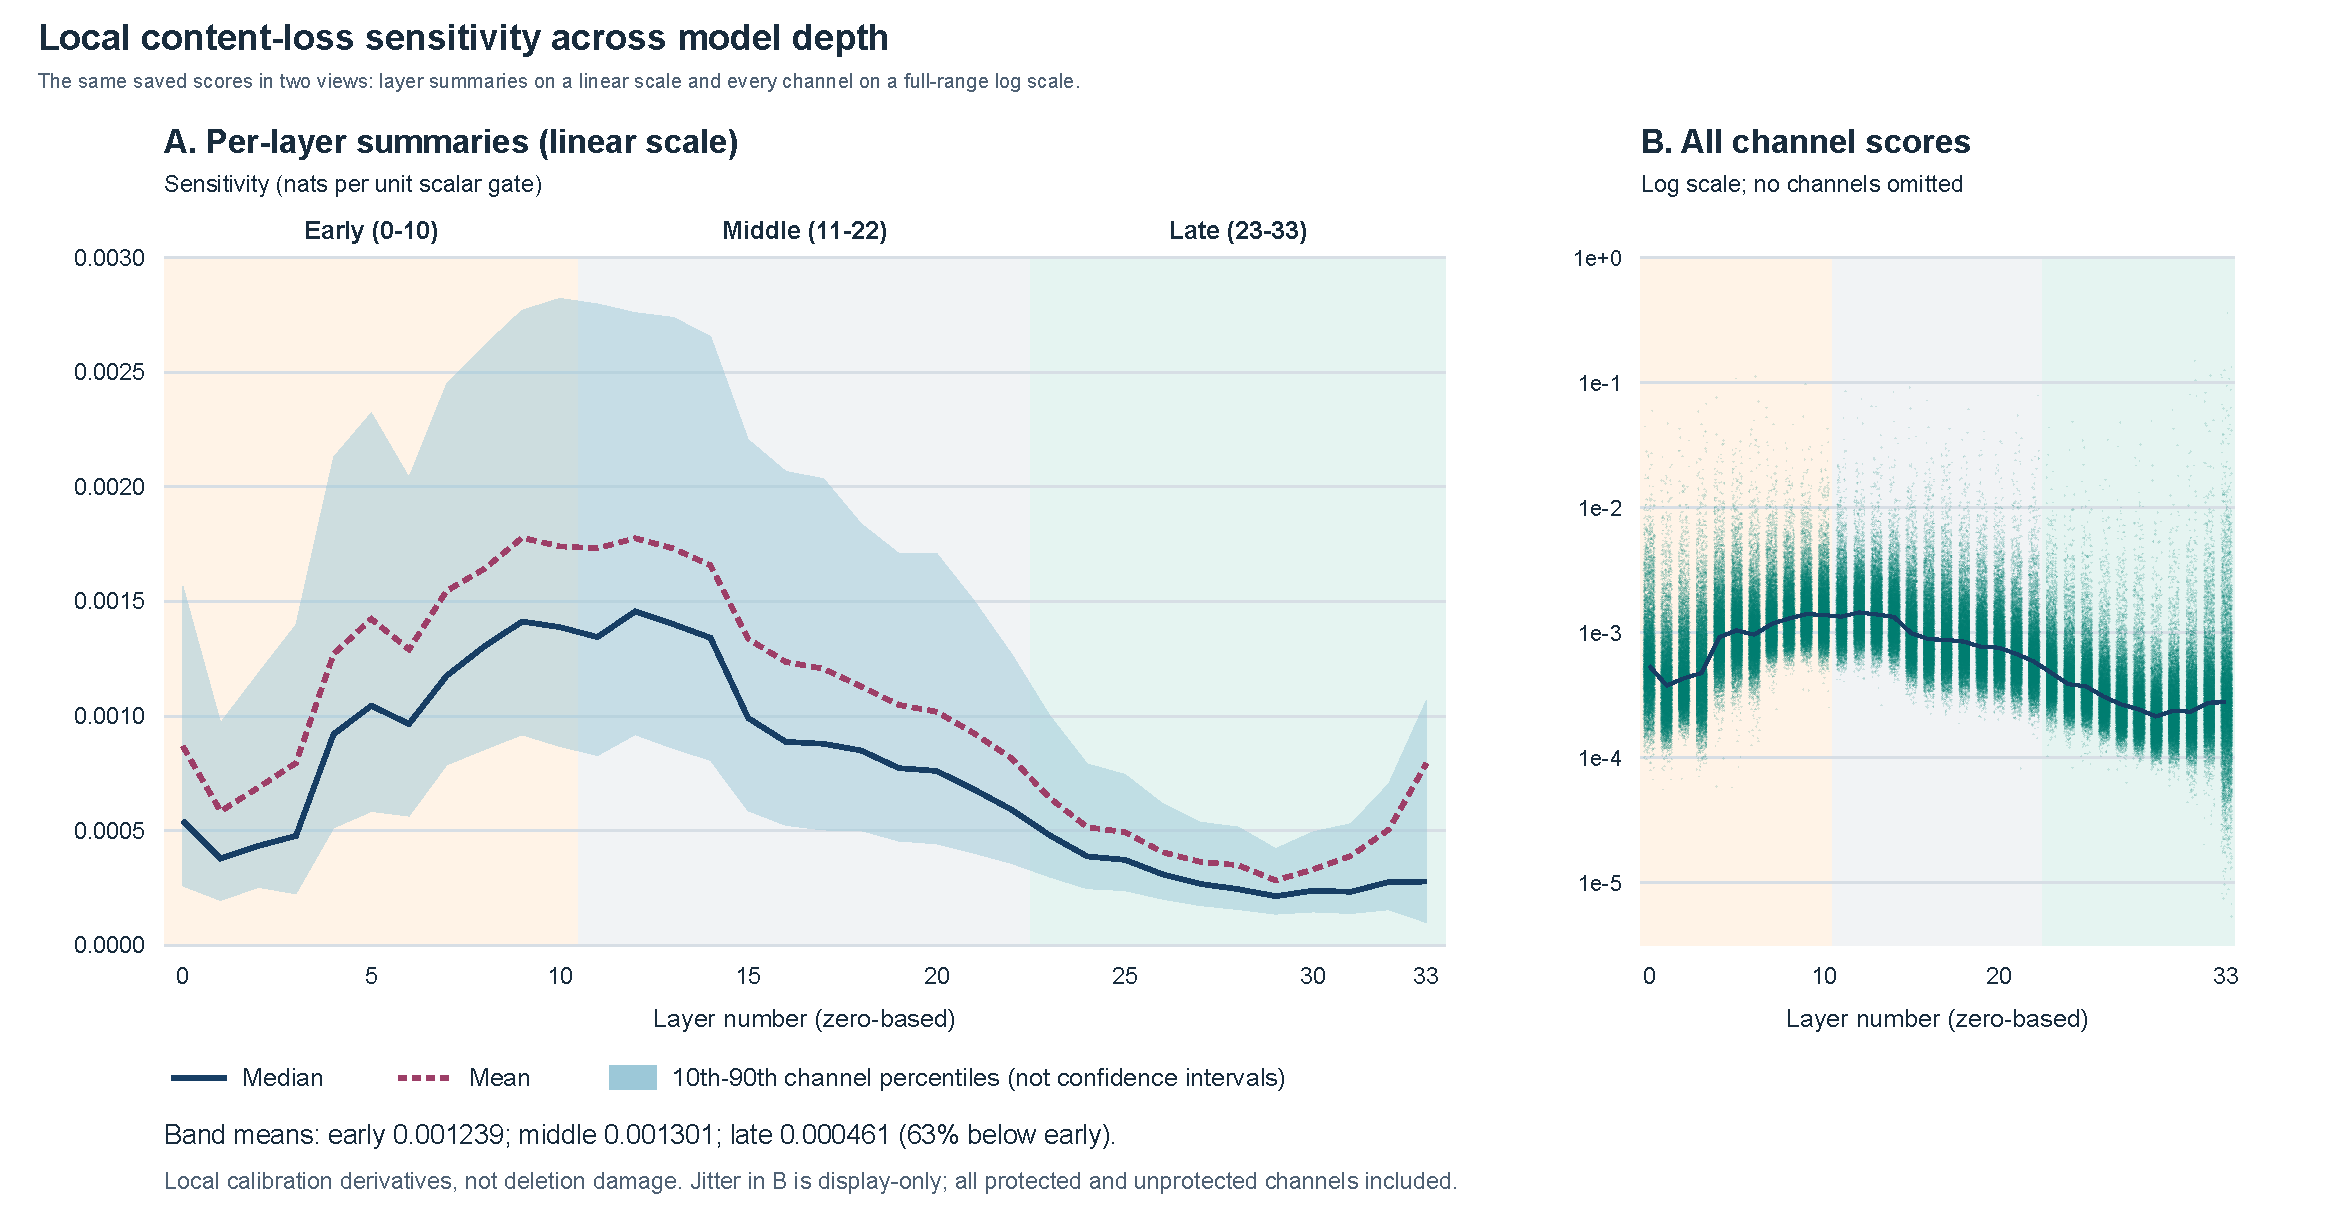
\includegraphics[width=\linewidth]{channel_loss_sensitivity_by_layer_v2.pdf}
\caption{Local content-loss sensitivity across depth, averaged equally
over 23 stored calibration strata (\dataset{D04}) using $S_{s,\mathrm{content},\ell j}$
from \autoref{eq:guided}. Left: linear-scale per-layer medians and means
with a shaded 10th--90th channel-percentile band, not a confidence interval.
Right: all 348,160 channel scores on a full-range logarithmic axis,
including protected channels, with display-only horizontal jitter and
the per-layer median. Both panels use the same raw scores, not
within-layer percentile ranks; local sensitivity is not deletion damage.}
\label{fig:channel-depth-sensitivity}
\end{figure}
\clearpage

\subsection{Quota-free guided selection}
\label{sec:quota-free-results}

Both quota-free interventions initially scored 14/128 on SQL (\dataset{D05}) and
0/64 on each graph task (\dataset{D05}). After matched LoRA, quota-free removal reached
98/128 SQL (\dataset{D05}) and quota-free reset 91/128, with validation NLL
(\dataset{D05}) 0.156758 and 0.157304 respectively.
Direct/two-step outcomes (\dataset{D05}) were 45/64 and 9/64
for removal, versus 32/64 and 12/64 for reset. The observed SQL
reset-minus-removal difference was $-5.47$ percentage points.
Quota-free removal scored $3.91$ points above both ordinary LoRA and
uniform guided removal. These single-seed observations motivate
replication of the recipe, not a universal winning-selector claim.

On the human-reviewed broad screen (\dataset{D06}), quota-free reset scored 62/120 and
quota-free removal 55/120, versus 64/120 for ordinary LoRA. Thus the
observed SQL advantage of quota-free removal did not carry over to the
broad scores. The changed selection objective and previously exposed
evaluation panels (\dataset{D05}, \dataset{D06})
limit attribution and generalization; equal or nearby
scores do not establish equivalence.

\begin{figure}[!htbp]
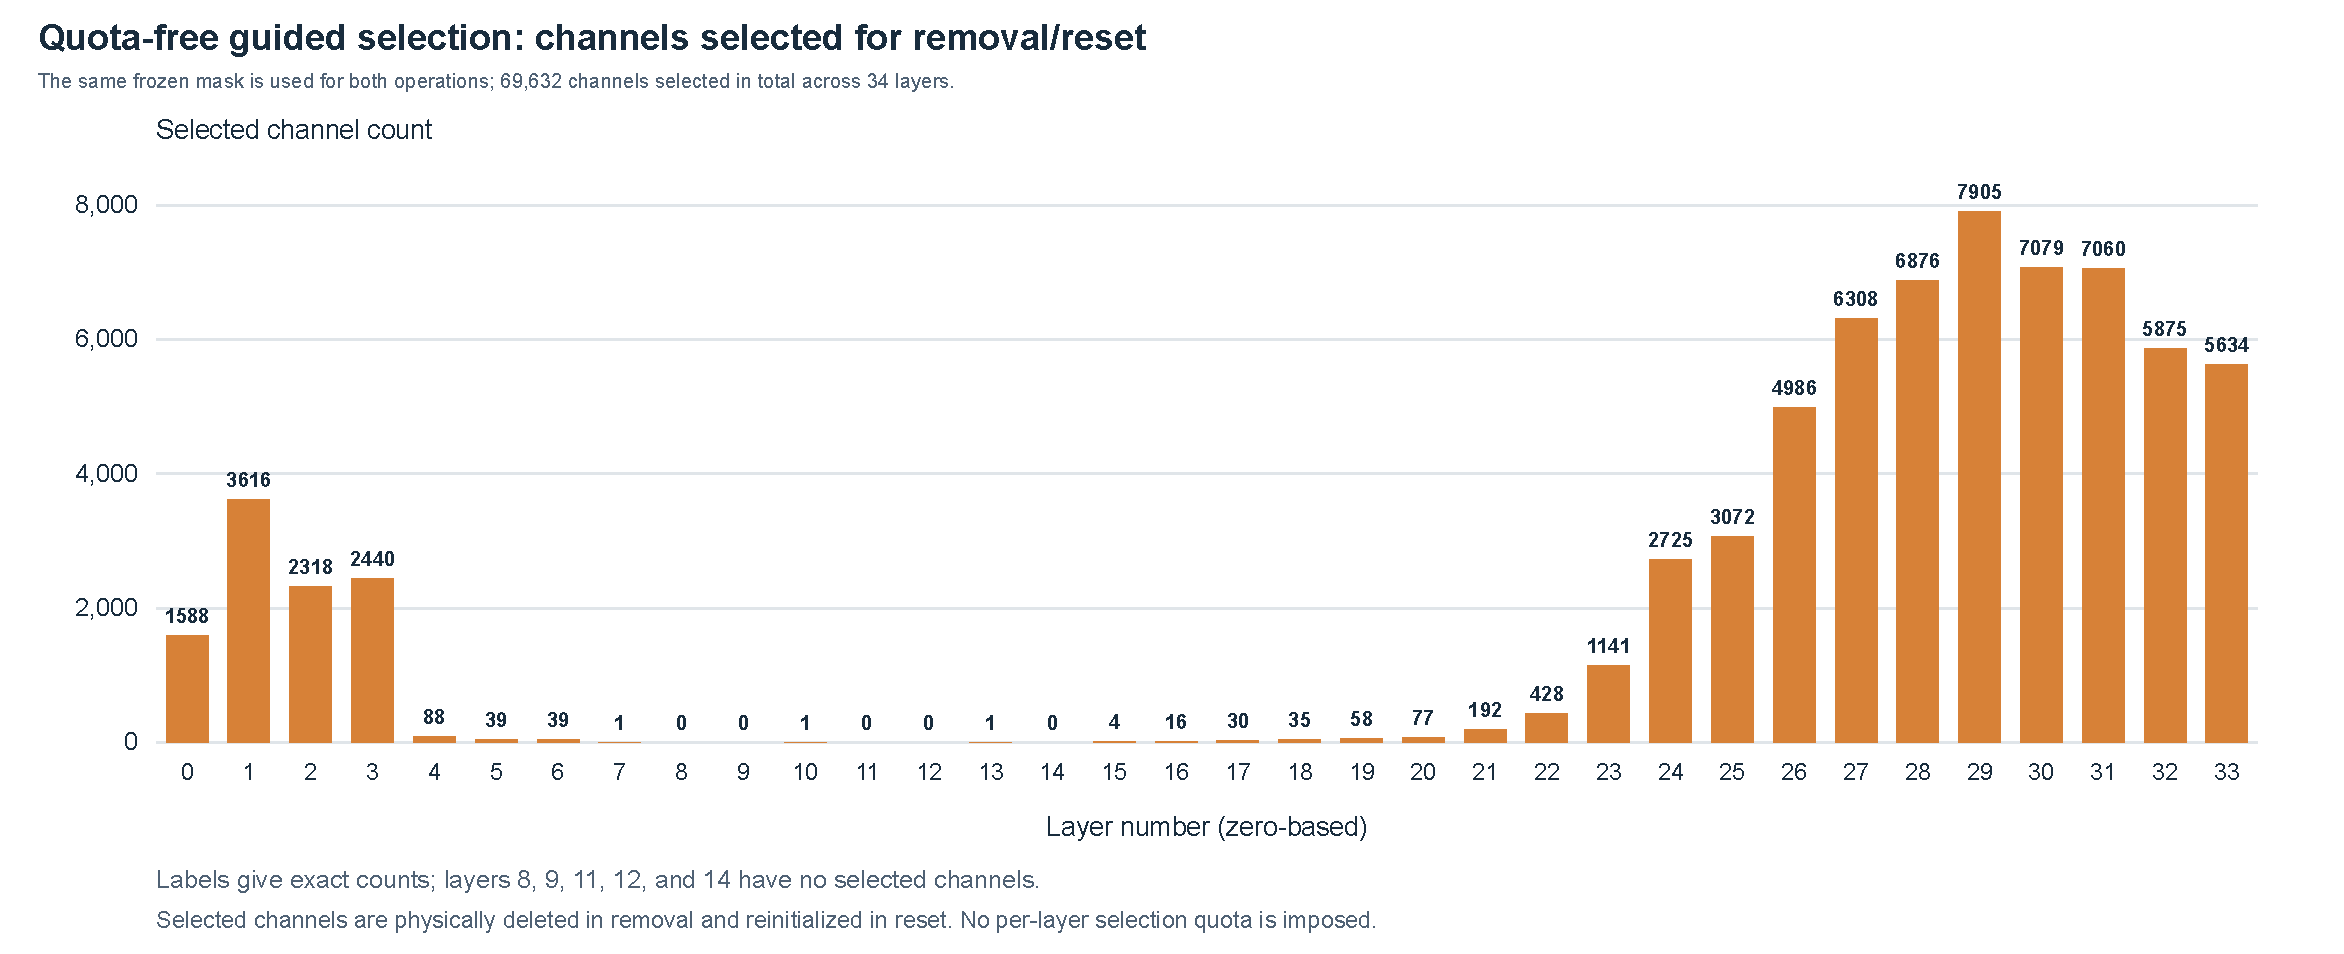
\includegraphics[width=\linewidth]{quota_free_selected_channels.pdf}
\caption{Channels selected for removal/reset in each layer by quota-free
guided selection. Bar labels give exact counts from the frozen mask,
totaling 69,632 across 34 layers of 10,240 original channels each.
Layers 8, 9, 11, 12, and 14 have no selected channels. The same coordinates
are physically deleted in removal and reinitialized in reset; all
explicitly protected channels are excluded from selection.}
\label{fig:guided-allocation}
\end{figure}
\section{Discussion and scope limitations}
\label{sec:discussion}

Against ordinary LoRA, quota-free guided removal offered a concrete trade-off: it 
used 13.78\% fewer native parameters and 10.5-10.8\% less peak training memory, 
while averaging 72.40\% SQL execution agreement versus 74.48\% across three 
matched seeds. Removal led on SQL in one seed and trailed in two, and it 
passed fewer broad-screen prompts in all three. The comparison among 
selection methods helps explain why quota-free guidance is nevertheless 
worth pursuing. At the same removal budget and training seed, SQL agreement 
rose from 88/128 with random selection to 90/128 with Taylor selection, 
93/128 with uniform guided selection, and 98/128 with quota-free guided selection; 
ordinary LoRA scored 93/128. The quota-free minus uniform guided removal
difference was $+3.91$ percentage points (paired 95\% interval:
$-2.59$ to $+10.29$; \autoref{app:paired-comparisons}). The interval permits
either ordering on SQL; the observed ranking does not establish superiority.
For reset, the clearest difference was on
the broad screen rather than SQL: quota-free guided reset passed 62/120 prompts, 
compared with 46--49/120 for the three uniform-allocation reset arms and 64/120 for ordinary
LoRA, but scored 91/128 on SQL versus ordinary LoRA's 93/128. These results make 
quota-free guidance a promising way to choose which channels to change under a 
fixed budget, not an established replacement for ordinary LoRA. The comparison 
among selectors used one training seed, one model, and one specialization task; 
moreover, the quota-free recipe changed both the scoring rule and how channels 
were allocated across layers. The evidence therefore motivates testing those two 
choices separately, rather than attributing the observed gains to removing layer 
quotas alone.

We deliberately bound the original nine-arm case study to one training seed,
with two additional seeds only for the ordinary-LoRA/quota-free-removal pair,
fixed masks and intervention budget, one pretrained model (Gemma 3 4B), and
text-to-SQL specialization. Three seeds for one pair do not establish
robustness across masks, models, domains, or the remaining arms. Adaptation uses LoRA with all native weights,
including reset weights, frozen, testing adapter-mediated reuse rather
than unrestricted relearning; removal and reset retain different parameter
capacities. Taylor and guided selection use different calibration sizes
(233 scoring examples in \dataset{D02} versus 437 in \dataset{D04}),
coverage, objectives, and selection compute, comparing complete recipes
rather than isolating the ranking algorithm. Quota-free removal/reset
keeps layerwise discovery protection (\dataset{D03}) fixed and changes
the ranking objective; global protection and allocation-only effects are
not tested. These intentional scope choices do not remove the qualifications
of development-exposed audits, single-instance SQL evaluation
(\dataset{D05}), the small AI-assisted broad screen (\dataset{D06}), or
shared-workstation measurements. Paired intervals describe evaluation
uncertainty, not retraining variability or general superiority.

\section{Conclusion and future work}
\label{sec:conclusion}
In this bounded case study, quota-free guided removal used 13.78\% fewer
native parameters and lower measured training-loop peak allocated CUDA memory.
Its original seed-42 SQL score (\dataset{D05}) of 98/128 exceeded ordinary
LoRA's 93/128, but two added seeds favored ordinary LoRA. The three-seed
comparison therefore does not show a consistent SQL advantage.
Selection and operation mattered jointly: guided selection did not
consistently outperform controls, and reset did not consistently outperform
removal. Quota-free reset instead had the highest broad-screen score
(\dataset{D06}) among the tabulated intervention arms, still trailing ordinary LoRA.
Each within-seed SQL interval for quota-free removal versus ordinary LoRA
included zero (\autoref{sec:seed-replication}). These observations make
quota-free removal a candidate for further study of compact specialization, 
not an established superior recipe, and leave the preferred removal/reset 
choice dependent on the evaluation objective.

Future work should extend training-seed replication to the remaining arms and replicate masks,
then extend the comparisons to other models and specialization domains. One important 
follow-up candidate is comparing uniform layerwise discovery protection with 
quota-free global allocation at fixed budgets. Matched calibration access and 
separately controlled ranking and allocation objectives would help isolate 
selector effects.

\paragraph{Reproducibility.}
\label{sec:reproducibility}
The GitHub repository at
\href{\repositoryurl}{\nolinkurl{https://github.com/adhasan-dev/remove-or-reset}} contains
project-authored data, pinned external-data acquisition and
preparation recipes, all reported channel masks, removal/reset code,
and scripts for LoRA training, evaluation, and numerical analysis.
The calibration-depth figure additionally requires numerical 
pre-intervention sensitivities, which are not bundled; frozen-mask retraining 
does not regenerate selectors. Environment specifications, configurations, checksums,
and usage instructions support reader-run reproduction. The initial
release does not include model weights, trained adapters, or historical
result evidence: readers will obtain the pinned Gemma base and external
data, run LoRA, and evaluate their trained models. Broad-screen scoring
(\dataset{D06}) requires independent human judgments and need not
exactly reproduce the published scores.

\label{page:core-end}
\clearpage
\bibliographystyle{plainnat}
\bibliography{references}

\clearpage
\appendix

\section{Selector definitions and supporting comparisons}
\label{app:selectors}
\subsection{How the channel masks were selected}

Each selector targets 69,632 MLP channels across 34 layers. A removal/reset
pair uses the same mask. Protection means excluding a coordinate from
selection, not simply retaining it in the final model.

\begin{center}
\small
\begin{tabular}{@{}lp{0.40\linewidth}ll@{}}
\toprule
Selector & Selection rule & Protected & Layer quota\\
\midrule
Random & Sample without replacement (seed 1042). & None & 2,048\\
Taylor & Lowest absolute gate derivative of target NLL, averaged within groups, then over groups and families. & None & 2,048\\
Uniform guided & Lowest worst within-layer percentile over strata and content/boundary losses. & 1,100 & 2,048\\
Quota-free guided & Lowest global score: equal-stratum mean of raw content sensitivities. & Same 1,100 & None\\
\bottomrule
\end{tabular}
\end{center}

For layer $\ell$ and channel $j$, a scalar gate $a_{\ell j}$ multiplies the
gated MLP activation at every token position. Let $\mathcal G_s$ be the groups
in stratum $s$, $\mathcal E_{sg}$ the examples in group $g$, and $\mathcal R_e$
the references for example $e$. For mean reference loss $L^{(k)}_{er}$ on
content or boundary tokens, guided sensitivity is
\begin{equation}
 S_{sk\ell j}=
 \frac{1}{|\mathcal G_s|}\sum_{g\in\mathcal G_s}
 \frac{1}{|\mathcal E_{sg}|}\sum_{e\in\mathcal E_{sg}}
 \left|\frac{1}{|\mathcal R_e|}\sum_{r\in\mathcal R_e}
 \left.\frac{\partial L^{(k)}_{er}}{\partial a_{\ell j}}\right|_{\boldsymbol a=\boldsymbol 1}\right|.
 \label{eq:guided}
\end{equation}
The signed reference derivatives are averaged \emph{before} taking the
absolute value. Quota-free selection averages $S_{s,\mathrm{content},\ell j}$
equally over 23 strata. Compared with uniform guidance, both the ranking
rule and the allocation across layers change; the protected set and total
channel budget do not.

\subsection{What the seed-42 comparisons establish}
\label{app:paired-comparisons}

\begin{center}
\small
\begin{tabular}{@{}lrr@{}}
\toprule
Comparison (first minus second) & SQL agreement & Broad Pass\\
\midrule
Quota-free vs.\ random removal & $+7.81\ [0.00,14.68]$ & $+7.50\ [-4.53,17.69]$\\
Quota-free vs.\ Taylor removal & $+6.25\ [-0.71,13.19]$ & $+5.00\ [-4.42,12.44]$\\
Quota-free vs.\ uniform guided removal & $+3.91\ [-2.59,10.29]$ & $+4.17\ [-5.32,12.51]$\\
Quota-free reset vs.\ quota-free removal & $-5.47\ [-10.53,-0.76]$ & $+5.83\ [-0.57,14.89]$\\
\bottomrule
\end{tabular}
\end{center}

Differences are percentage points with descriptive paired 95\% intervals
(\autoref{sec:uncertainty}). Quota-free removal scored above all three
removal alternatives on both panels, but every selector interval includes
zero. At the same quota-free mask, removal had the higher SQL score and
reset the higher broad Pass count. These within-seed intervals do not
measure variation across training seeds or masks.

\end{document}
